\documentclass{article}

\usepackage{geometry}
\usepackage{amsmath}
\usepackage{graphicx, eso-pic}
\usepackage{listings}
\usepackage{hyperref}
\usepackage{multicol}
\usepackage{fancyhdr}
\pagestyle{fancy}
\fancyhf{}
\hypersetup{ colorlinks=true, linkcolor=black, filecolor=magenta, urlcolor=cyan}
\geometry{ a4paper, total={170mm,257mm}, top=40mm, right=20mm, bottom=20mm, left=20mm}
\setlength{\parindent}{0pt}
\setlength{\parskip}{0.5em}
\renewcommand{\headrulewidth}{0pt}
\AddToShipoutPictureBG{%
  \AtPageUpperLeft{%
    \raisebox{-\height}{
\includegraphics[width=\paperwidth, height=30mm]{../headerarkav.png}}
  }
}
\rfoot{\thepage}
\lfoot{Competitive Programming - Arkavidia 8.0}
\lstset{
    basicstyle=\ttfamily\small,
    columns=fixed,
    extendedchars=true,
    breaklines=true,
    tabsize=2,
    prebreak=\raisebox{0ex}[0ex][0ex]{\ensuremath{\hookleftarrow}},
    frame=none,
    showtabs=false,
    showspaces=false,
    showstringspaces=false,
    prebreak={},
    keywordstyle=\color[rgb]{0.627,0.126,0.941},
    commentstyle=\color[rgb]{0.133,0.545,0.133},
    stringstyle=\color[rgb]{01,0,0},
    captionpos=t,
    escapeinside={(\%}{\%)}
}

\begin{document}

\begin{center}
    \section*{I. Isekai} % ganti judul soal

    \begin{tabular}{ | c c | }
        \hline
        Batas Waktu  & 1s \\    % jangan lupa ganti time limit
        Batas Memori & 256MB \\  % jangan lupa ganti memory limit
        \hline
    \end{tabular}
\end{center}

\subsection*{Deskripsi}
Pada suatu hari yang cerah, Arka sedang berjalan santai sambil memikirkan cara untuk masuk isekai. Namun saat Arka hendak menyebrangi jalan, tiba-tiba saja Arka tertabrak oleh Truk-kun.

Arka kemudian terbangun dan bertanya-tanya apakah Arka sudah berada di isekai? Lalu, tiba-tiba terdengar suara aneh yang berkata “Selamat datang! Kamu sedang berada di permainan ‘Tebak Isekai’." 

Pada permainan ini, hanya ada 1 portal menuju isekai dari $N$ portal yang ada. Permainan diawali dengan Arka memilih salah satu portal. Kemudian, terdapat $K$ ronde yang di setiap rondenya akan dihancurkan 1 portal yang bukan merupakan portal pilihan Arka dan juga bukan portal menuju isekai. Arka juga berkesempatan untuk mengganti pilihan portal pada setiap ronde dengan memilih portal lain yang belum hancur atau tetap dengan pilihannya.

Setelah permainan selesai, Arka pun masuk ke dalam portal yang terakhir Arka pilih. Jika Arka bermain secara maksimal, tentukanlah probabilitas tertinggi Arka masuk isekai!

\subsection*{Format Masukan}
Baris pertama terdiri dari dua bilangan bulat $N$ ($1 \leq N \leq 10^9$) dan $K$ ($0 \leq K < N$).

\subsection*{Format Keluaran}
Keluarkan satu baris terdiri dari dua bilangan bulat $P$ dan $Q$ yang dipisahkan oleh spasi, menyatakan probabilitas tertinggi Arka masuk isekai ialah $\frac{P}{Q}$ dimana $P$ relatif prima terhadap $Q$.

\begin{multicols}{2}
\subsection*{Contoh Masukan 1}
\begin{lstlisting}
3 1
\end{lstlisting}
\columnbreak

\subsection*{Contoh Keluaran 1}
\begin{lstlisting}
2 3
\end{lstlisting}
\vfill
\null
\end{multicols}

\begin{multicols}{2}
\subsection*{Contoh Masukan 2}
\begin{lstlisting}
5 2
\end{lstlisting}
\columnbreak

\subsection*{Contoh Keluaran 2}
\begin{lstlisting}
2 5
\end{lstlisting}
\vfill
\null
\end{multicols}

\subsection*{Penjelasan}
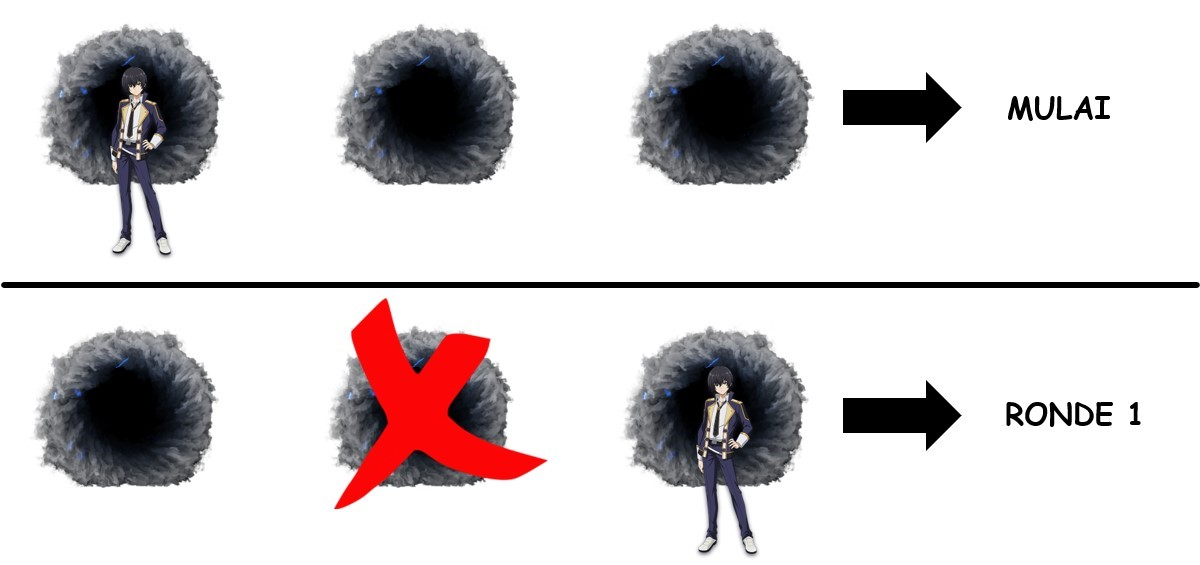
\includegraphics[width=225px]{Contoh_Tebak_Isekai.jpg}

Pada contoh masukan pertama, terdapat 3 portal dan 1 ronde. Pada awal permainan, Arka memilih portal ke-1. Lalu pada ronde 1, portal ke-2 dihancurkan dan Arka pindah ke portal ke-3. Setelah permainan selesai, Arka masuk ke portal ke-3 dan probabilitas Arka masuk isekai ialah $\frac{2}{3}$. Ini merupakan probabilitas tertinggi dan dapat dibuktikan tidak ada cara lain untuk memperoleh probabilitas lebih tinggi lagi.

\end{document}